  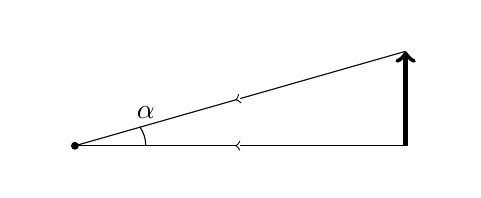
\begin{tikzpicture}[scale=0.6]
    \clip (-1,-0.5) rectangle (8,2.5) ; %Les dimensions de l'image

    \filldraw [black] (0,0) circle (2pt) node [left] {$\ptO$} ;  %Point O
    
      \draw [->,ultra thick] (7,0) node at (7.5,0) {$\ptA$} -- (7,2) node at (7.5,2) {$\ptB$} ;   %L'objet

      \draw [-<,thin] (0,0) -- (3.5,1)  ; 
      \draw [-,thin] (3.5,1) -- (7,2) ; %Le rayon lumineux reliant B et O
      
      \draw [-<,thin] (0,0) -- (3.5,0) ; %Le rayon lumineux reliant A et O
      \draw [-,thin] (3.5,0) -- (7,0) ; %Le rayon lumineux reliant A et O
       
      \draw (1.5,0) arc (0:35:20pt) node at (1.5,0.7) {$\alpha$} ;  %Repérage angle
      
  \end{tikzpicture}